\begin{exercice}
Voici le nombre de points obtenus dans une épreuve commune de mathématiques.

\begin{tabular}{|l|l|}
\hline
Nombre de points & Nombres d'élèves \\ \hline
10               & 2                \\ \hline
9                & 7                \\ \hline
8                & 11               \\ \hline
7                & 17               \\ \hline
6                & 14               \\ \hline
5                & 12               \\ \hline
4                & 8                \\ \hline
3                & 5                \\ \hline
2                & 3                \\ \hline
1                & 1                \\ \hline
\end{tabular}

Établir le tableau statistique complet. Précision des calculs dans le tableau : 4 chiffres après la virgule.
Établir l'histogramme des effectifs et des fréquences cumulées.
Indiquer le mode et la médiane de cette distribution statistique.
Calculer la moyenne et l'écart-type.
S'il faut avoir 6 points pour avoir la moyenne à cet examen, calculer le pourcentage d'élèves qui ont alors obtenu au minimum la note 4.
\end{exercice}

\begin{exercice}
On a relevé dans ce tableau la vitesse de 125 voitures sur l'autoroute.

\begin{tabular}{|l|l|l|l|l|l|l|l}
\hline
136 & 132 & 137 & 120 & 130 & 108 & 147 & \multicolumn{1}{l|}{136} \\ \hline
142 & 134 & 109 & 120 & 130 & 128 & 142 & \multicolumn{1}{l|}{131} \\ \hline
142 & 135 & 105 & 95  & 131 & 98  & 127 & \multicolumn{1}{l|}{116} \\ \hline
156 & 111 & 114 & 108 & 133 & 118 & 108 & \multicolumn{1}{l|}{146} \\ \hline
120 & 127 & 106 & 132 & 98  & 163 & 115 & \multicolumn{1}{l|}{117} \\ \hline
117 & 167 & 127 & 135 & 113 & 115 & 124 & \multicolumn{1}{l|}{118} \\ \hline
132 & 110 & 114 & 134 & 115 & 134 & 112 & \multicolumn{1}{l|}{141} \\ \hline
135 & 124 & 119 & 175 & 119 & 102 & 151 & \multicolumn{1}{l|}{128} \\ \hline
116 & 114 & 118 & 111 & 129 & 133 & 130 & \multicolumn{1}{l|}{125} \\ \hline
124 & 124 & 123 & 118 & 105 & 120 & 123 & \multicolumn{1}{l|}{118} \\ \hline
148 & 126 & 116 & 113 & 112 & 117 & 134 & \multicolumn{1}{l|}{106} \\ \hline
119 & 107 & 143 & 140 & 128 & 131 & 137 & \multicolumn{1}{l|}{122} \\ \hline
123 & 125 & 160 & 157 & 99  & 116 & 120 & \multicolumn{1}{l|}{117} \\ \hline
125 & 152 & 108 & 121 & 115 & 125 & 145 &                          \\ \cline{1-7}
110 & 153 & 107 & 132 & 128 & 98  & 116 &                          \\ \cline{1-7}
122 & 121 & 145 & 116 & 102 & 125 & 125 &                          \\ \cline{1-7}
\end{tabular}

On demande de trier les résultats en classe de 10 km/h, puis de recopier et de compléter le tableau ci-dessous.

\begin{landscape}

\begin{tabular}{llllllll}
\cline{1-1}
\multicolumn{1}{|l|}{\begin{tabular}{l}Vitesse mesurée (en km/h)\\ de 125 véhicules \\ sur l'autoroute\end{tabular}} &                                &                                &                                &                                &                                  &                                &                                   \\ \hline
\multicolumn{1}{|l|}{Classes}                                                    & \multicolumn{1}{l|}{Centre}    & \multicolumn{1}{l|}{Effectifs} & \multicolumn{1}{l|}{Fréquence} & \multicolumn{1}{l|}{Fréquence} & \multicolumn{1}{l|}{Fréquence}   & \multicolumn{1}{l|}{Fréquence} & \multicolumn{1}{l|}{Fréquence}    \\ \hline
\multicolumn{1}{|l|}{(en km/h)}                                                  & \multicolumn{1}{l|}{de classe} & \multicolumn{1}{l|}{}          & \multicolumn{1}{l|}{}          & \multicolumn{1}{l|}{cumulée}   & \multicolumn{1}{l|}{cumulée inv} & \multicolumn{1}{l|}{pondérée}  & \multicolumn{1}{l|}{pond. carrée} \\ \hline
\multicolumn{1}{|l|}{{]}90 - 100{]}}                                             & \multicolumn{1}{l|}{}          & \multicolumn{1}{l|}{}          & \multicolumn{1}{l|}{}          & \multicolumn{1}{l|}{}          & \multicolumn{1}{l|}{}            & \multicolumn{1}{l|}{}          & \multicolumn{1}{l|}{}             \\ \hline
\multicolumn{1}{|l|}{{]}100 - 110{]}}                                            & \multicolumn{1}{l|}{}          & \multicolumn{1}{l|}{}          & \multicolumn{1}{l|}{}          & \multicolumn{1}{l|}{}          & \multicolumn{1}{l|}{}            & \multicolumn{1}{l|}{}          & \multicolumn{1}{l|}{}             \\ \hline
\multicolumn{1}{|l|}{{]}110 - 120{]}}                                            & \multicolumn{1}{l|}{}          & \multicolumn{1}{l|}{}          & \multicolumn{1}{l|}{}          & \multicolumn{1}{l|}{}          & \multicolumn{1}{l|}{}            & \multicolumn{1}{l|}{}          & \multicolumn{1}{l|}{}             \\ \hline
\multicolumn{1}{|l|}{{]}120 - 130{]}}                                            & \multicolumn{1}{l|}{}          & \multicolumn{1}{l|}{}          & \multicolumn{1}{l|}{}          & \multicolumn{1}{l|}{}          & \multicolumn{1}{l|}{}            & \multicolumn{1}{l|}{}          & \multicolumn{1}{l|}{}             \\ \hline
\multicolumn{1}{|l|}{{]}130 - 140{]}}                                            & \multicolumn{1}{l|}{}          & \multicolumn{1}{l|}{}          & \multicolumn{1}{l|}{}          & \multicolumn{1}{l|}{}          & \multicolumn{1}{l|}{}            & \multicolumn{1}{l|}{}          & \multicolumn{1}{l|}{}             \\ \hline
\multicolumn{1}{|l|}{{]}140 - 150{]}}                                            & \multicolumn{1}{l|}{}          & \multicolumn{1}{l|}{}          & \multicolumn{1}{l|}{}          & \multicolumn{1}{l|}{}          & \multicolumn{1}{l|}{}            & \multicolumn{1}{l|}{}          & \multicolumn{1}{l|}{}             \\ \hline
\multicolumn{1}{|l|}{{]}150 - 160{]}}                                            & \multicolumn{1}{l|}{}          & \multicolumn{1}{l|}{}          & \multicolumn{1}{l|}{}          & \multicolumn{1}{l|}{}          & \multicolumn{1}{l|}{}            & \multicolumn{1}{l|}{}          & \multicolumn{1}{l|}{}             \\ \hline
\multicolumn{1}{|l|}{{]}160 - 170{]}}                                            & \multicolumn{1}{l|}{}          & \multicolumn{1}{l|}{}          & \multicolumn{1}{l|}{}          & \multicolumn{1}{l|}{}          & \multicolumn{1}{l|}{}            & \multicolumn{1}{l|}{}          & \multicolumn{1}{l|}{}             \\ \hline
\multicolumn{1}{|l|}{{]}170 - 180{]}}                                            & \multicolumn{1}{l|}{}          & \multicolumn{1}{l|}{}          & \multicolumn{1}{l|}{}          & \multicolumn{1}{l|}{}          & \multicolumn{1}{l|}{}            & \multicolumn{1}{l|}{}          & \multicolumn{1}{l|}{}             \\ \hline
                                                                                 & \multicolumn{1}{l|}{}          & \multicolumn{1}{l|}{}          & \multicolumn{1}{l|}{}          &                                & \multicolumn{1}{l|}{}            & \multicolumn{1}{l|}{}          & \multicolumn{1}{l|}{}             \\ \cline{3-4} \cline{7-8} 
\end{tabular}

\end{landscape}

Établir l'histogramme des fréquences et des fréquences cumulées.
Indiquer la valeur de la classe modale et de la classe médiane.
Calculer la vitesse moyenne et l'écart-type.
Calculer le pourcentage de véhicules qui roulent à une vitesse supérieure à la vitesse autorisée en Suisse.
\end{exercice}

\begin{exercice}
Afin d'analyser les habitudes de la clientèle d’un supermarché, le gérant a relevé les montants des achats faits par les clients un lundi après-midi et un samedi après-midi.

\begin{tabular}{lll|l|l|}
\cline{1-2} \cline{4-5}
\multicolumn{1}{|l|}{Lundi aprčs-midi} & \multicolumn{1}{l|}{}         &  & Samedi aprčs-midi &          \\ \cline{1-2} \cline{4-5} 
\multicolumn{1}{|l|}{Classe}           & \multicolumn{1}{l|}{Effectif} &  & Classe            & Effectif \\ \cline{1-2} \cline{4-5} 
\multicolumn{1}{|l|}{{]}0 - 20{]}}     & \multicolumn{1}{l|}{7}        &  & {]}0 - 20{]}      & 5        \\ \cline{1-2} \cline{4-5} 
\multicolumn{1}{|l|}{{]}20 - 40{]}}    & \multicolumn{1}{l|}{16}       &  & {]}20 - 40{]}     & 12       \\ \cline{1-2} \cline{4-5} 
\multicolumn{1}{|l|}{{]}40 - 60{]}}    & \multicolumn{1}{l|}{32}       &  & {]}40 - 60{]}     & 23       \\ \cline{1-2} \cline{4-5} 
\multicolumn{1}{|l|}{{]}60 - 80{]}}    & \multicolumn{1}{l|}{24}       &  & {]}60 - 80{]}     & 48       \\ \cline{1-2} \cline{4-5} 
\multicolumn{1}{|l|}{{]}80 - 100{]}}   & \multicolumn{1}{l|}{10}       &  & {]}80 - 100{]}    & 61       \\ \cline{1-2} \cline{4-5} 
\multicolumn{1}{|l|}{{]}100 - 120{]}}  & \multicolumn{1}{l|}{7}        &  & {]}100 - 120{]}   & 34       \\ \cline{1-2} \cline{4-5} 
\multicolumn{1}{|l|}{{]}120 - 140{]}}  & \multicolumn{1}{l|}{3}        &  & {]}120 - 140{]}   & 29       \\ \cline{1-2} \cline{4-5} 
\multicolumn{1}{|l|}{{]}140 - 160{]}}  & \multicolumn{1}{l|}{1}        &  & {]}140 - 160{]}   & 14       \\ \cline{1-2} \cline{4-5} 
                                       &                               &  & {]}160 - 180{]}   & 12       \\ \cline{4-5} 
                                       &                               &  & {]}180 - 200{]}   & 6        \\ \cline{4-5} 
                                       &                               &  & {]}200 - 220{]}   & 4        \\ \cline{4-5} 
                                       &                               &  & {]}220 - 240{]}   & 2        \\ \cline{4-5} 
\end{tabular}

Il te demande d'établir, pour chaque après-midi étudiée, un tableau statistique (montants des achats groupés en classes de vingt francs), de calculer le mode, la médiane, la moyenne des dépenses et l'écart-type. Il souhaite aussi connaître le pourcentage des clients dont le montant des achats est égal ou inférieur à Fr. 60.–– et le pourcentage de ceux dont le montant est strictement supérieur à Fr. 100.—. Précision des calculs : trois chiffres après la virgule.
Avec les résultats obtenus, le gérant du supermarché te demande encore de faire, pour chaque après-midi, un commentaire sur les habitudes d'achat de la clientèle (justifier les commentaires en utilisant les divers paramètres statistiques calculés !). Il souhaite aussi que tu trouves quelques raisons sociologiques aux différences observées.
\end{exercice}

\begin{exercice}
On a mesuré la longueur en millimètres des grains de deux variétés de riz. Les résultats des mesures ont été répertoriés dans le tableau annexé.

\begin{tabular}{|l|l|l|}
\hline
                         & Variété A & Variété B \\ \hline
Taille des grains de riz & Effectif  & Effectif  \\ \hline
{]}0  2{]}               & 7         & 2         \\ \hline
{]}2 - 4{]}              & 37        & 5         \\ \hline
{]}4 - 6{]}              & 72        & 28        \\ \hline
{]}6 - 8{]}              & 89        & 98        \\ \hline
{]}8 - 10{]}             & 97        & 230       \\ \hline
{]}10 - 12{]}            & 91        & 107       \\ \hline
{]}12 - 14{]}            & 69        & 25        \\ \hline
{]}14 - 16{]}            & 34        & 4         \\ \hline
{]}16 - 18{]}            & 4         & 1         \\ \hline
\end{tabular}

\begin{enumerate}
\item Pour chaque variété de riz, établir un tableau de statistiques complet. 
	Précision des calculs : trois chiffres après la virgule.
\item Pour chacune des deux variétés de riz, on souhaite connaître :
	\begin{itemize}
	\item La classe modale,
	\item Le pourcentage des effectifs que représente la classe modale à elle seule,
	\item Le pourcentage des grains ayant une mesure inférieure ou égale à 8 mm,
	\item Le pourcentage des grains ayant une mesure strictement supérieure à 10 mm,
	\item La classe médiane,
	\item La moyenne,
	\item L’écart-type.
	\end{itemize}
\item Procéder à une analyse des résultats statistiques obtenus puis comparer les deux variétés de riz.
\item Pour commercialiser le riz, on procède à un tri mécanique qui élimine à la fois les grains dont la taille est inférieure ou égale à 6 millimètres et les grains dont la taille est strictement supérieure à 14 millimètres. Quelle variété de riz se prêtera le mieux à la commercialisation, justifier votre réponse ? 
\end{enumerate}
\end{exercice}


\begin{exercice}
Voici trois exemples de distribution statistique. Commenter chacune de ces distributions avec les renseignements fournis par les histogrammes, les modes, les médianes, les moyennes et les écarts-types. Donner un exemple d''étude d'un caractère d'une population qui aurait le même genre de distribution.
\begin{center}
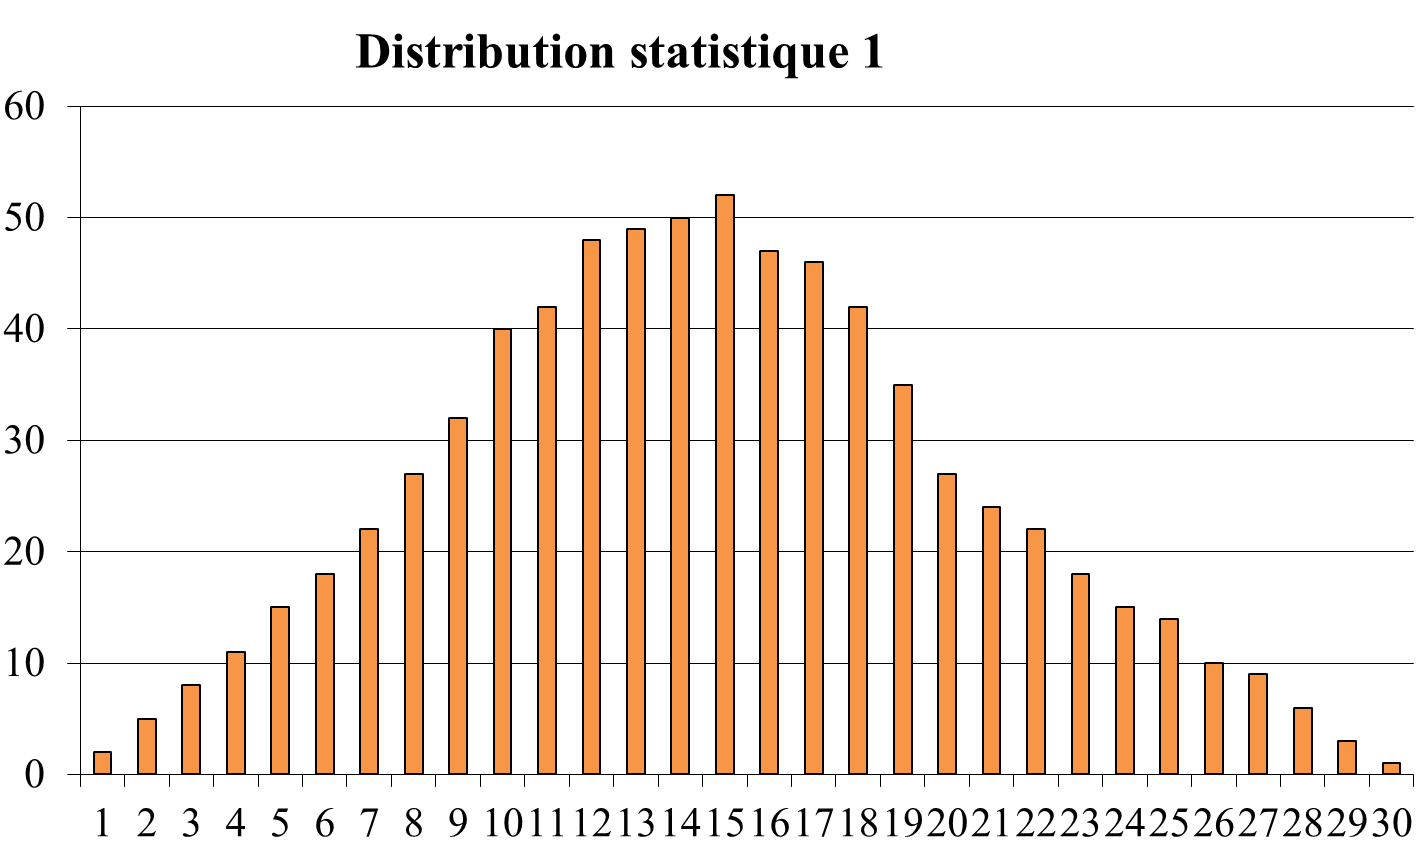
\includegraphics[width = 0.5\textwidth]{statistiques/image/graphique1.png}
\end{center}
Mode : 15
Médiane : 15
Moyenne : 14.69
Écart-type : 5.78
\begin{center}
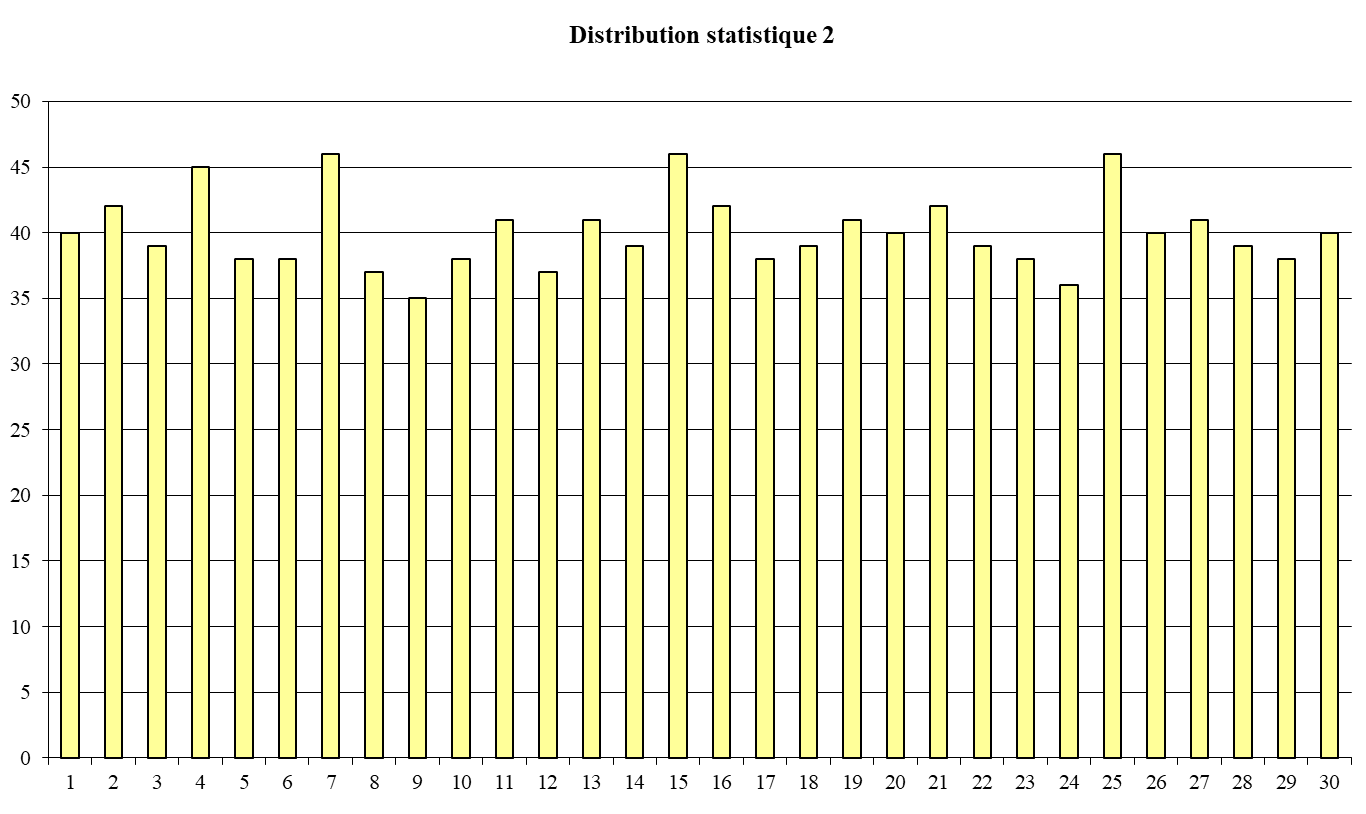
\includegraphics[width = 0.5\textwidth]{statistiques/image/graphique2.png}
\end{center}
Mode : 5
Médiane : 13
Moyenne : 14.77
Écart-type : 9.44
\begin{center}
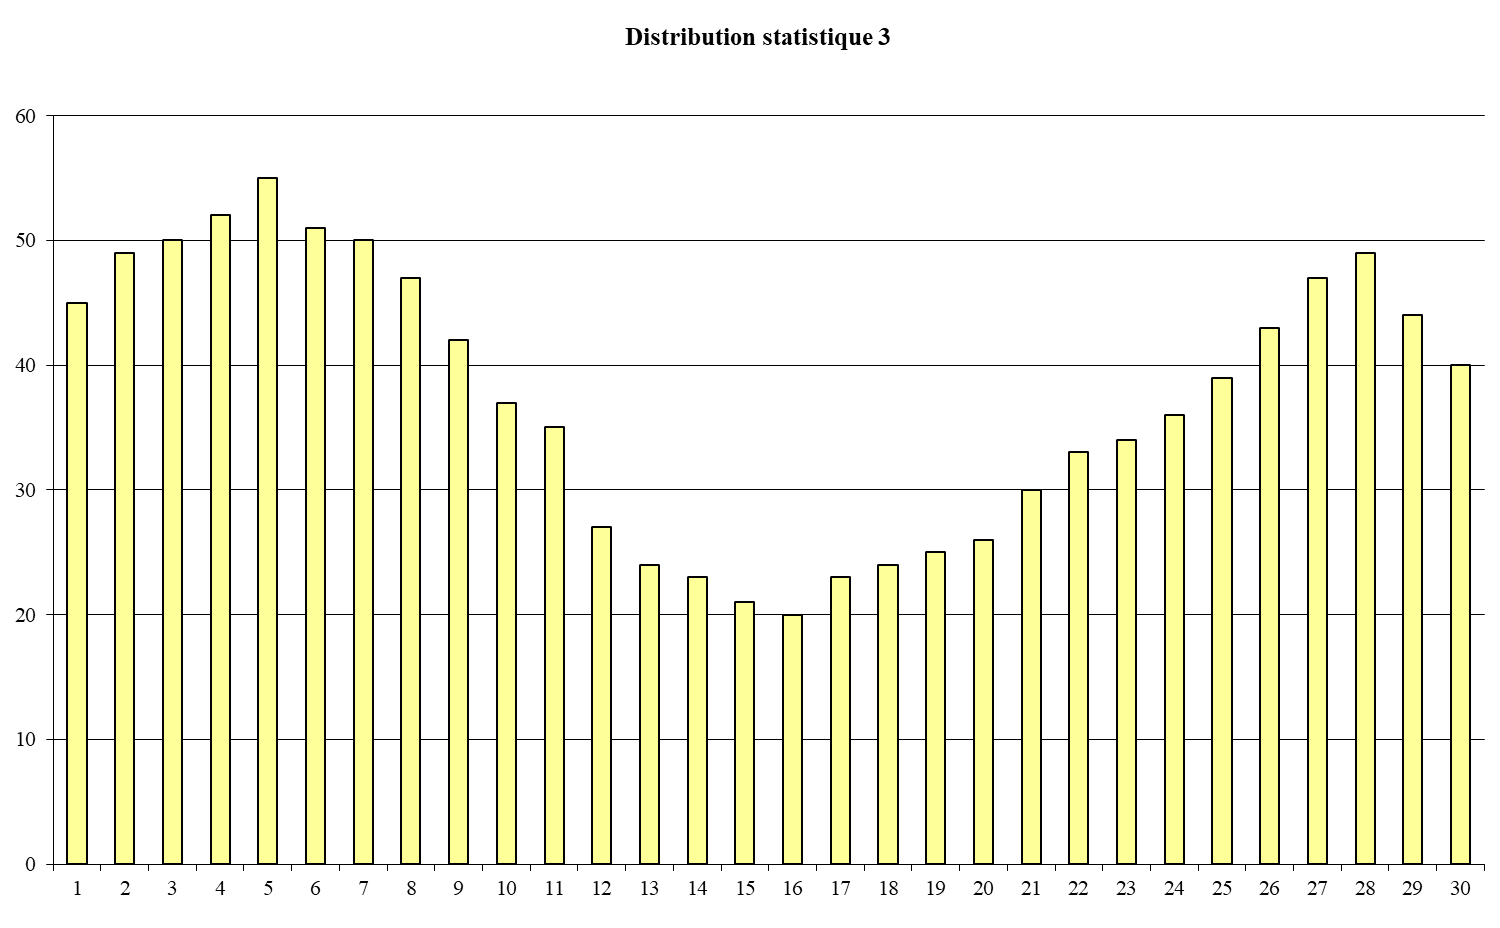
\includegraphics[width = 0.5\textwidth]{statistiques/image/graphique3.png}
\end{center}
Mode : 7 – 15 - 25
Médiane : 15
Moyenne : 15.47
Écart-type : 8.66
\end{exercice}

\begin{exercice}
Dans le tableau suivant, on a répertorié le nombre de repas servis à midi dans un restaurant. Calculer l'équation de la droite de régression linéaire et le coefficient de corrélation. Commenter les résultats obtenus.

\begin{tabular}{|l|l|l|l|l|l|l|l|}
\cline{1-2} \cline{4-5} \cline{7-8}
Jour (x) & Repas (y) &  & Jour (x) & Repas (y) &  & Jour (x) & Repas(y) \\ \cline{1-2} \cline{4-5} \cline{7-8} 
1        & 12        &  & 11       & 16        &  & 21       & 31       \\ \cline{1-2} \cline{4-5} \cline{7-8} 
2        & 10        &  & 12       & 15        &  & 22       & 22       \\ \cline{1-2} \cline{4-5} \cline{7-8} 
3        & 13        &  & 13       & 17        &  & 23       & 24       \\ \cline{1-2} \cline{4-5} \cline{7-8} 
4        & 12        &  & 14       & 25        &  & 24       & 15       \\ \cline{1-2} \cline{4-5} \cline{7-8} 
5        & 11        &  & 15       & 15        &  & 25       & 23       \\ \cline{1-2} \cline{4-5} \cline{7-8} 
6        & 14        &  & 16       & 18        &  & 26       & 24       \\ \cline{1-2} \cline{4-5} \cline{7-8} 
7        & 20        &  & 17       & 20        &  & 27       & 21       \\ \cline{1-2} \cline{4-5} \cline{7-8} 
8        & 13        &  & 18       & 16        &  & 28       & 33       \\ \cline{1-2} \cline{4-5} \cline{7-8} 
9        & 8         &  & 19       & 22        &  & 29       & 19       \\ \cline{1-2} \cline{4-5} \cline{7-8} 
10       & 15        &  & 20       & 20        &  & 30       & 24       \\ \cline{1-2} \cline{4-5} \cline{7-8} 
\end{tabular}
\end{exercice}

\begin{exercice}
Un exploitant d'une épicerie pense qu'il existe une relation linéaire entre le nombre de clients et le jour de la semaine. Calculer l'équation de la droite de régression linéaire, le coefficient de corrélation, puis confirmer ou infirmer l'impression de l'exploitant.

\begin{tabular}{|l|l|l|l|l|l|l|l|}
\hline
Jour (x)              & Lundi & Mardi & Mercredi & Jeudi & Vendredi & Samedi & Dimanche \\ \hline
Nombre de clients (y) & 146   & 206   & 146      & 133   & 156      & 202    & 124      \\ \hline
\end{tabular}
\end{exercice}

\begin{exercice}
Le tableau suivant donne le prix de vente x (en francs) et la quantité y vendue d'un objet au cours des douze derniers mois.

\begin{tabular}{|l|l|l|l|l|l|l|l|l|l|l|l|l|}
\hline
Prix (x)     & 6  & 5  & 4   & 6  & 8  & 4   & 7  & 5   & 6  & 9  & 3   & 3   \\ \hline
Quantité (y) & 75 & 92 & 102 & 85 & 60 & 115 & 70 & 105 & 88 & 30 & 141 & 127 \\ \hline
\end{tabular}


Calculer l'équation de la droite de régression linéaire et le coefficient de corrélation linéaire.
Représenter le nuage de points et la droite de régression sur un même graphique. 
Unité des axes : abscisse 1 cm pour un franc, ordonnée 1 cm pour 10 objets
Selon ce modèle de régression, quel serait la quantité d'objets vendus pour un prix de vente de Fr. 10.— ?
Selon ce modèle de régression, à quel prix correspondrait une vente de 100 objets ?
\end{exercice}